
\documentclass[12pt,a4paper,english]{article}
\usepackage{graphicx, csquotes, babel, multicol, multirow, amssymb, fullpage, amsmath, tabularx}
\usepackage[utf8]{inputenc}
\inputencoding{utf8}
\usepackage[T2A]{fontenc}
\usepackage[table]{xcolor}
\MakeOuterQuote{"}
\begin{document}

\title{Analysis of knowledge requirements for text alignment problem}
\author{Bartosz Kalińczuk}
\date{\today}
\maketitle

\newpage
\begin{abstract}
The purpose of this final master degree project was to experiment with various algorithms for speech and text alignment either with granularity of sentences, single words or even single phonemes. The output of this study was expected to find out how little data is necessary to compute a proper alignment. This project focuses mainly on Polish language, however it can be quite easily generalized for different languages. It also focuses solely on a audio with quite low level of noise, since  it introduces a lot of problems, and is out of the scope of this project.
\end{abstract}


\newpage
\setcounter{tocdepth}{2}
\tableofcontents

\newpage
\section{Introduction}

\newpage
\begin{center}
    \section{Speech signal}
\end {center}
\subsection{Human factor}

Speech is a most efficient way the human communicate. For generations this process was refined by evolution, so we can easily exchange messages even in hard situations. For this purpose our vocal mechanisms must well cooperate with our hearing ability. There is a certain set of sounds we can produce and our ears evolved to hear them as well as possible.\newline 

What is sound? According to dictionary: "Vibrations transmitted through an elastic solid or liquid or gas, with frequencies in the approximate range of 20 to 20000 hertz, capable of being detected by human organs of hearing". [1]\newline

How do we hear? Human ear consist about 30000 hair-cells, which can convert mechanical wave of the sound into electromagnetic wave inside auditory nerves [2]. 
Each of these cell is excited by different frequency of mechanical wave of internal ear fluids, so it is no surprise, that people can hear only a certain range of frequencies, as stated in definition. These we expect to be finely tuned to the range of the sounds we can produce. Although it seems, that we can hear a bit more, but as we don't need that, it happens, that as we grow older, our hearing range is getting smaller, because our hear cells fail sometimes, but mostly those responsible for high frequencies, which we don't use too often.\newline

Humans can hear frequencies, that begins as low as 12Hz (under laboratory conditions) to 20kHz (for adults usually much lower). However speech range is a little bit smaller than that [3]: \newline

\begin{center}
    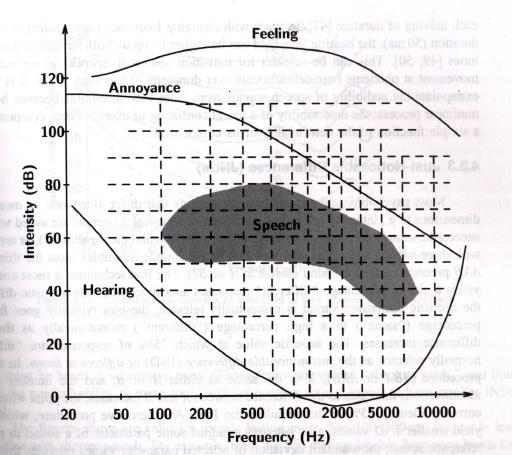
\includegraphics[scale=0.5]{speech_range.jpg}
\end {center}


\newpage
\subsection{Mel scale}

How we perceive sound, that is completely different matter and topic for long philosophical discussion. However we can help ourselves with some subjective experiments. For example Stevens, Volkman and Newman conducted an experiment on a number of listeners to measure, what do we perceive as equally distanced pitches. In this experiment, the participants of the experiment were asked to judge if given pitches were in equal distances. The output was, that humans don't experience sound linearly respectively to the frequency scale, but a perceptual scale was closer to logarithmic one. [5] \newline

Certain formulas were conceived to translate frequency scale to one, that is closer to how human actually perceive sound. \newline

One popular is mel scale, where mel comes from melody: [6] \newline
\begin{equation}
    m = 2595log_{10}(1 + \frac{f}{700})
\end{equation}
	
What looks like that:
\begin{center}
    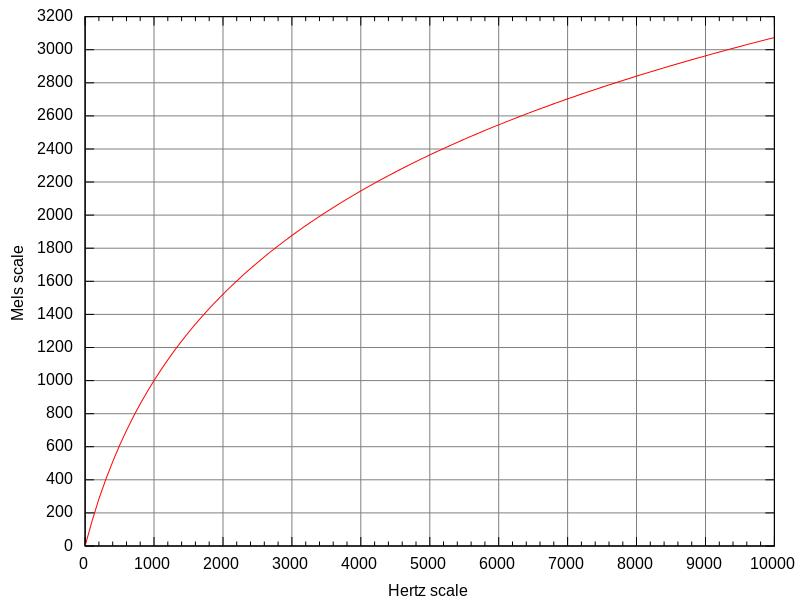
\includegraphics[scale=0.3]{mel_scale.jpg}
\end {center}

Another popular formula of so called bark scale, which is based on perception of loudness of the sound and proposed by Eberhard Zwicker in 1961. [7] \newline
\begin{equation}
    Bark = 13 atan(\frac{0.76f}{1000}) + 3.5 atan(\frac{f^2}{7500^2})
\end{equation}
In this project we use mel scale implemented in sphinx library, although bark scale is becoming more popular recently.

\newpage
\subsection{Frequency spectrum}

The conclusion from the anatomy of human ear is, that frequencies of the sound are important.
How can we obtain frequency spectrum from a digitized sound, so we can proceed further? \newline
The obvious tool for conversion of discrete function to frequencies is Discrete Fourier Transform, named after Jean Baptiste Joseph Fourier it is one of the most often used techniques of modern times. \newline

It all started from the postulate, that a heat equation can be satisfied by function of form: [11] \newline
\begin{equation}
    f(x)=\sum_{n=0}^N(A_n cos(nx) + B_n sin(nx))
\end{equation}
or in complex form:
\begin{equation}
    f(\theta)=\sum_{n=-\infty}^{\infty} C_n e^{i n \theta}
\end{equation}

Basically we convert our function's domain to frequency domain or to domain of sinusoidal functions. $C_n$ coefficients are complex values that encode both amplitude and phase of the converted signal/function at each frequency. \newline

The coefficients for any integrable functions over an interval $[\frac{-T}{2}, \frac{T}{2}]$ can be obtain using formula: [11] \newline
\begin{equation}
    C_n=\int_{\frac{-T}{2}}^{\frac{T}{2}} f(x) e^{-2 \pi i \frac{n}{T} x} dx
\end{equation}

or for the discrete case:
\begin{equation}
    C_k=\sum_{n=0}^{N-1} x_n e^{\frac{-2 \pi i k n}{N}} dx
\end{equation}
	

So far we haven't found any use in the speech recognition for phase part of the coefficients, however amplitude determines how powerful is signal at given frequency. The power value is given by:
\begin{equation}
    |X_k|/N = \sqrt{\Re(X_k)^2 + \Im(X_k)^2} / N
\end{equation}

\newpage
A sample conversion:
\begin{center}
    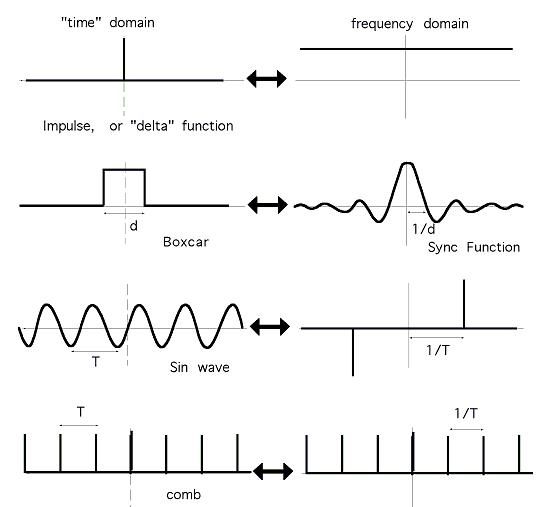
\includegraphics[scale=0.3]{sample_dft_conversion.jpg}
\end {center}

What size of the window should we use? First we have to notice, that in order to capture certain frequency, the window needs to be large enough. We would like to examine signals of frequency ranged from 100Hz (see speech frequencies ranges in chapter 2.1), which is a period of 100th of the second, so a 10millisecond window would be our bottom limit. \newline

Also windows with abrupt signal discontinuities may cause result with spectral artefacts, so a windowing function is usually applied. Popular choice is a Hamming window function: [8]
\begin{equation}
   w_j = 0.54 - 0.46 cos(\frac{2 \pi j}{W - 1}) 
\end{equation}
Which's plot is:
\begin{center}
    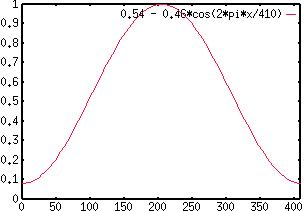
\includegraphics[scale=0.3]{hamming_window.jpg}
\end {center}

Note that it emphasises values in the middle of the window, so our actual windows should overlap to cover whole time domain. For example by shifting a window by a percentage of it actual width:
\begin{center}
    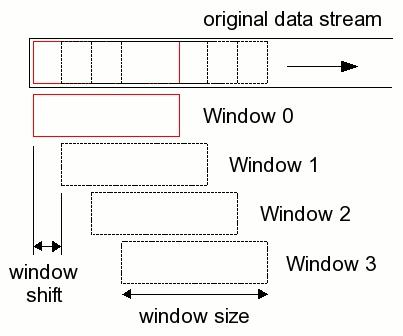
\includegraphics[scale=0.3]{window_shifting.jpg}
\end {center}

\newpage
A human speech signal in frequency and time domain: [3]
\begin{center}
    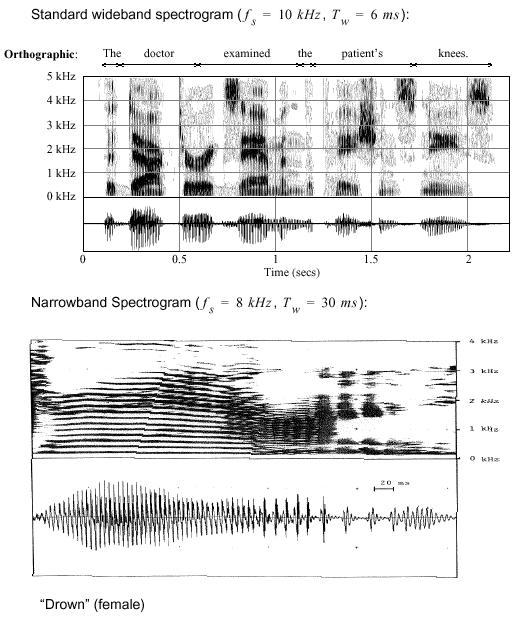
\includegraphics[scale=0.8]{speech_spectrogram.jpg}
\end {center}

\newpage
\subsection{Cepstrum}

Looking at the frequency spectrum of human speech we see, that  the signal in the frequency domain contain features that are quite periodic. As it is with converting initial signal with DFT, we would like to extract the information of periodicity in the spectrum. 
A cepstrum of the signal gives us this additional information. \newline

The word is derived by reordering characters in the word spectrum to indicate switch of domains, similarly as word 'quefrency'. The cepstrum operates in the domain of time and the basic intuition is, that it reveals a rate of change in the different spectrum bands. 
For example a cepstrum of an echoed signal in the picture below shows clearly a three 'quefrencies' of the echo of the signal. [12]
\begin{center}
    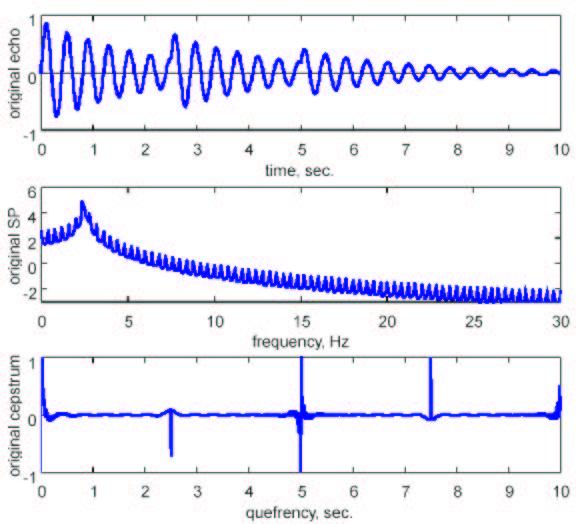
\includegraphics[scale=0.4]{echo_cepstrum.jpg}
\end {center}


Cepstrum definition is: "Inverse Fourier transform of the logarithm of the magnitude of the Fourier transform" or:
\begin{equation}
    C=|F^{-1}{log(|F{f(t)}|^2)}|^2
\end{equation}

,or:
\begin{equation}
    c_x[n] = \frac{1}{2\pi} \int_{-\pi}^{\pi}log |X(e^{j \omega})| e^{j \omega n} d\omega
\end{equation}

This is the definition of the power cepstrum, since it is calculated from the magnitude of each frequency band. However there also exists a complex, real and phase cepstrum depending on what part of initial Fourier transform it uses.
In speech related problems a power cepstrum is usually used and I haven't see any reason to not focus only on this.


\newpage
\addtolength{\textwidth}{4cm}
This is a typical cepstrum sequence of the vowel [3] computed every 10ms. \newline

\begin{minipage}[-100,0]{5cm}
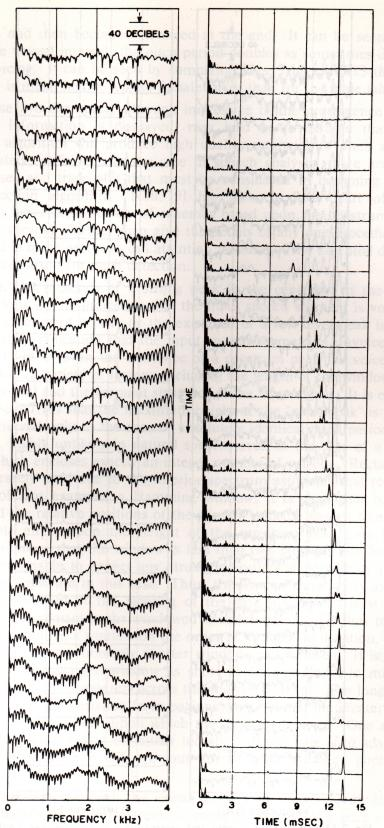
\includegraphics[width=5cm,height=21cm]{vowel_cepstrum.jpg}
\end{minipage}
\begin{minipage}[5cm,0]{9cm}

If the sound becomes periodic in the frequency domain it's quefrency domain contains a peak which is related to the periodicity of the sound. \newline

Note that similar results can be obtained by taking just additional DFT of the signal. Inverse Fourier Transform is closely related to Fourier Transform and also performs a split of the function into periodic components. \newline
\newline
After all IFT is defined:
\begin{equation}
     f(x) = \int_{\mathbb{R} ^ n} e^{2 i \pi x \zeta} \hat{f}(\zeta) d\zeta
\end{equation}
while FT is defined: 
\begin{equation}
    \hat{f}(\zeta) = \int_{\mathbb{R} ^ n} f(x) e^{-2 i \pi \zeta x} dx
\end{equation}

Why taking logarithm of the magnitude? It serves as a normalization of power spectrum. In speech for example it happens, that low frequency components are usually more powerful than high frequncy components and by normalizing the signal, the periodicity becomes more apparent. \newline


A bit different way of looking at the signal cepstrum is as a homomorphic transformation which changes convolution into sum. [3]
\begin{equation}
x(n) = e(n) * h(n)
\end{equation}
\begin{equation}
\hat x(n) = \hat e(n) + \hat h(n)
\end{equation}


Which on it's own can be seen as way of separating signals, since it is more easy to extract elements from a sum, than from a convolution.
\newline
\newline
In the example with echo, we could have used the cepstrum to separate echoed signal from initial signal, and it might be used to filter out an audio feedback.

\end{minipage}

\newpage
\subsection{Sphinx frontend}


Sphinx is a speech recognition toolkit with a lot of useful functionalities for any speech related problem.  \newline
There is a certain common way to prepare a speech signal for the further processing. With slight variations in each step, the useful informations about speech are drawn from a cepstrum of the reduced signal (in the number of data dimensions), as presented in this chapter. \newline

In order to skip the reinvention of the wheel, I used the fronted part of the sphinx library in any experiment in this project.
The sphinx fronted performs signal transformation and produces data composed of only 39 voice features,
while actually only 13 are base ones and the rest is a derivation of these. \newline

Sphinx frontend is a list of transformations executed on the result of the transformation placed higher in the list.
In another words it is a transformation composition. \newline
\newline
This Sphinx frontend pipeline includes: \newline
\begin{itemize}
	\item Data Blocker,
	\item Preemphasizer,
	\item Windower,
	\item Discrete Fourier Transform,
	\item Mel Frequency Filter Bank,
	\item Discrete Cosine Transform,
	\item Cepstral Mean Normalization,
	\item Deltas Feature Extractor.
\end{itemize}

\subsubsection{Data Blocker}

This initial transformation reads incoming double data read from audio source (file or microphone) and
prepares blocks of the data to be used in later phases. In our case blocks contain 10ms of audio data.

\subsubsection{Preemphasizer}

The Preemphasizer applies a formula: $Y[i]=x[i]-(X[i-1] * preemphasizerFactor)$.
The purpose of this transformation is to emphasize the high frequency components. It is kind of filter,
which allows high frequency components to pass through, but weakens the low frequency ones.


\newpage
\subsubsection{Raised cosine windower}

Creates windows from the incoming data. A windowing function
\begin{equation}
    W(n)=(1-\alpha) - \alpha cos(\frac{2 \pi n}{N - 1})
\end{equation}
 is applied afterwards. Alpha coefficient set to 0.46 results with a mentioned before Hamming windowing
 function, which is a default setting and the one used by me.

\subsubsection{Discrete Fourier Transform}

Implementation of fast Fourier transform .The FFT can perform transformation with complexity $\Omega(Nlog(N))$,
where N is the size of the input data.
It can be perform on whole data, however in speech we would like to get an information of the frequencies 
of a small frame, that contains consistent speech signal, in particular a single phoneme.
The output data is the power spectrum of input data window and the complex/phase information is lost.
The number of FFT points is the closest power of 2 equal or larger to the number of samples in the incoming window of data. However the input signal is real, so resulting FFT is symmetric, so only half of the data is returned and the output size is $\frac{FFT points}{2} + 1$.

\subsubsection{Mel frequency filter bank}

This step is a part of calculating a Mel Frequency Cepstrum. \newline

Conversion of frequency spectrum into a mel-spectrum using triangular overlapping windows defined as:
\begin{equation}
    w(n) = 1 - |\frac{n - (N - 1)/2}{(N + 1)/2}|
\end{equation}


The number of triangles/filters defined the size of mel-spectrum and the sphinx's default is 40. \newline
The filters are chosen, so the result would simulate a mel-scale given by the formula:
\begin{equation}
    melFreq = 2595 log(1 + linearFrequency / 700)
\end{equation}

The given filters should look like in the picture:
\begin{center}
    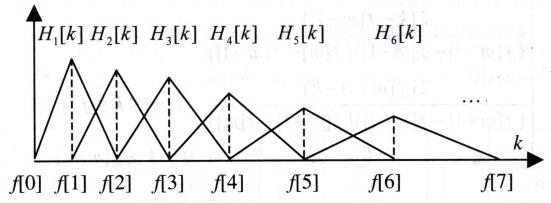
\includegraphics[scale=0.4]{mel_filters.jpg}
\end {center}

Not all frequencies are covered by the filters.
The chosen range of frequencies may differ for various audio encodings,
but generally should cover only the speech ranges.
The default values for 16kHz sample rate streams are 130Hz-6800Hz and are not changed in this project.

\newpage
\subsubsection{Discrete Cosine Transform}

Another part of calculating Mel Frequency Cepstral Coefficient vector.  \newline

It applies a logarithm and the DCT type II to the input data.  \newline

A DCT type II (most common) coefficients are defined as: 
\begin{equation}
    C(u) = \alpha(u)\sum_{x=0}^{N-1} f(x)cos[\frac{\pi(2x+1)u}{2N}] 
\end{equation}
and it is quite tightly related to real part of the Fourier Transform. [18]
The transform represents a function as a sum of cosine functions and it is equivalent to the DFT operating
real data with even symmetry. \newline
The number of dimensions returned is set by default to 13.

\subsubsection{Cepstral Mean Normalization}

Performs a normalization of MFCC vector by subtracting a mean of all the input. There are two versions
of this step. One that calculates mean online and the other that reads all data before performing
subtraction.

\subsubsection{Deltas feature extractor}

The final transformation in the sphinx frontend chain. It calculates first and second order derivative of the
cepstrum as additional features of the speech signal. It improves noticeable speech processing algorithms
by adding additional information about changes in the cepstrum data. \newline

For the initial cepstrum data it adds additionally twice the size vector with first and second order
differences, calculated as shown in the picture:
\begin{center}
    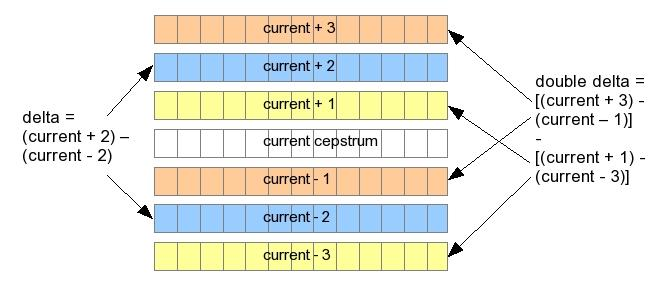
\includegraphics[scale=0.6]{deltas_calc.jpg}
\end {center}

\newpage
\begin{center}
    \section{Speech Modelling}
\end {center}
\setcounter{equation}{0}

\subsection{Phones, phonemes and graphemes}

A phone is a unit of speech sound [20]. Phoneme's definition is: "The smallest contrastive linguistic unit, which may bring about a change of meaning" [21], so the phoneme is a classification unit of phones, which allow us to represent speech while preserving its meaning.  While speech is being modelled using phonemes the graphical part of the language in form of text is modelled with characters or graphemes. \newline

Language grapheme set usually differs quite substantially from it audio counterparts. Often it contains more characters than needed to represent every word from given language and at the same time it is much too small to represent all the nuances of human speech. What is more problematic, the word graphic representation often has very little to do with actual phones of the word. I.e. there are so called homographes: words, that are written the same yet they pronunciation differs ("zamarzać" from "marznąć" and "morzyć") or homophones, that look differently, but are pronounced similar ("może", "morze"). In polish though, the former is quite rare and this fact is actually used by me (chapter 5.3). \newline


Actual phones that are classified under single phoneme create a diversified family.  Different variants of a phoneme are called allophones. For example /l/ in English "leap" and "deal" or polish examples of allophones (/ł/ in "umysł" might be soundless contrary to "ławka") or vowels between soft consonants (/a/ in "jajko"). [22] \newline

The phonemes can differ quite substantially depending on the surrounding phones. For example almost each phoneme in polish changes to softer version when put next to /i/ or /j/. Consecutive phones are not necessarily separated by clearly visible moment of silence. Often one phone is converting slowly into another. To model such a transitions a diphones or triphones are modelled for each sequence of two or three phones. \newline

Phonemes are very important in the computational language modelling, either in speech recognition or alignment. The importance is derived directly from its definition. It is a unit of speech, which can't be switched to another without changing the meaning. This is the unit, that need to be modelled if we want to recognize and/or distinguish different words. Finer granularity of model is necessary only to make a better prediction where an observed phone belongs.

\newpage
Some of English phonemes and example phones:
\begin{center}
    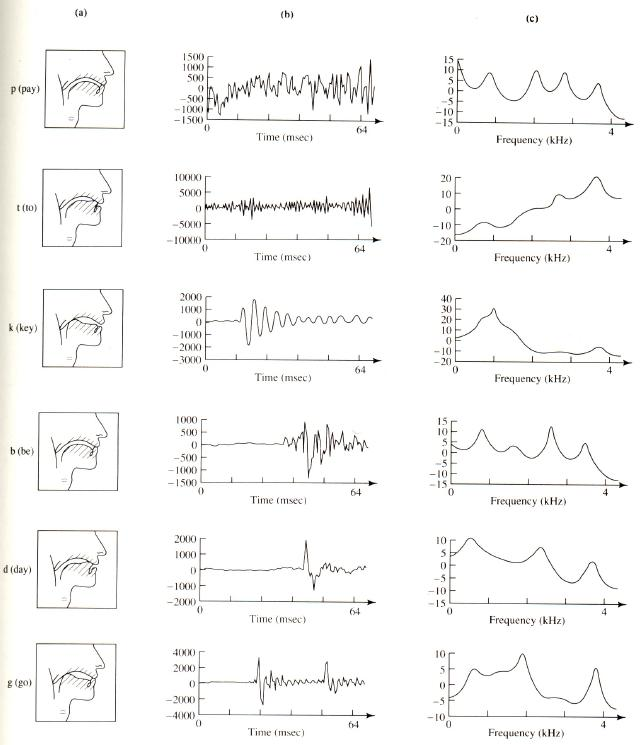
\includegraphics[height=11cm, width=16cm]{example_phones_1.jpg}
    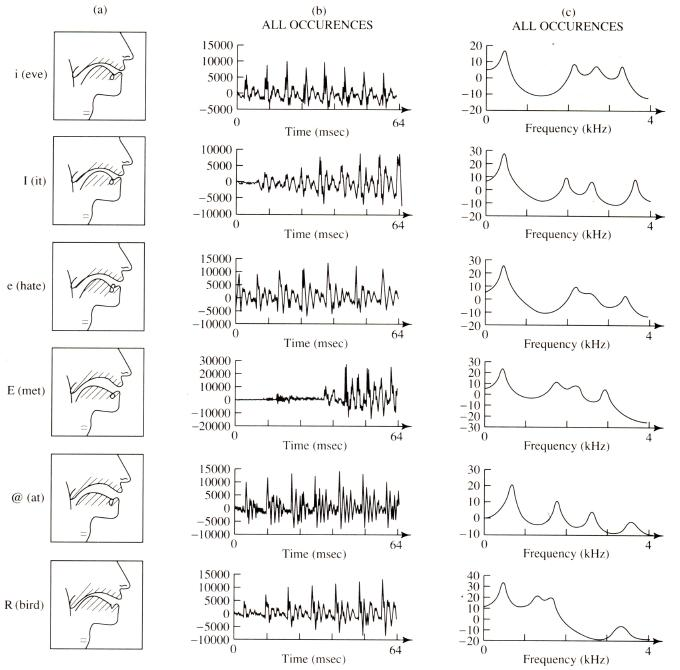
\includegraphics[height=11cm, width=16cm]{example_phones_2.jpg}
\end {center}

\newpage
\subsection{Audio distances}

The simplest way to find similar audio sequence is to find a sequence which is nearby to another,
that we know represents a certain sound, phoneme or word. \newline

To calculate a distance we could use various norms:
\begin{equation}
    ||x||_1 , || x ||_2, ... , || x ||_\infty
\end{equation}
, where 
\begin{equation}
    ||x||_k = (\sum_{i=0}^{N} x_i^k)^\frac{1}{k}
\end{equation}
and they are all fine for uncorrelated vectors, which is not really our case. \newline


For correlated vectors, we could try to introduce some weighting factor inside.\newline
What factor should we use?\newline
One approach is to tune the factors using external methods, which theoretically may give us some additional benefit of properly modelling phonemes, that we try to measure distance from, however this is a bit out of the scope of this chapter and most probably would in the end look similar to a different method.
A simpler approach would be to calculate correlations and use them in a distance measure.
If we had a correlation matrix ($P$) and than our distance could be:
\begin{equation}
    dist_{using correlations}(\vec x, \vec p) = (\vec x - \vec p)^T P^{-1} (\vec x - \vec p)
\end{equation}
               
Karl Pearson introduced such an idea [23] in form of correlation coefficient defined between two random populations:  
\begin{equation}
    \rho_XY = \frac{cov(X, Y)}{\sigma_X \sigma_Y} = \frac{E[(X - \mu_X)(Y - \mu_Y)]}{\sigma_X \sigma_Y}
\end{equation}
and in the form of matrices:  
\begin{equation}
    P = (\Sigma^{diagonal})^{-1/2} \Sigma (\Sigma^{diagonal})^{-1/2}
\end{equation}

It should be noted, that in the denominator we have standard deviations which don't really bring any value to our measure, since this is a constant factor.
By removing them we obtain so called Mahalanobis distance [16]:
\begin{equation}
    distance_{Mahalanobis}(\vec x, \vec p) = (\vec x - \vec p)^T \tilde C^{-1} (\vec x - \vec p)
\end{equation}

If we knew elements belonging to any given phoneme, we could calculate a distance between this training sample and any encounter speech signal.

\newpage

I conducted couple of experiments with different distances.
Starting with a flawed alignment of larger portions of text I tried to:
\begin{itemize}
	\item find the same word, that is quite lengthy and occurs multiple times just by searching for similar sequences,
	\item find a given sequence of three phonemes in a text, based on estimated location (time)
\end{itemize}

Mahalanobis distance in those experiments where not expected to any give significant results,
since there were conducted without knowledge of phone classification and it behaved without a surprise. \newline


The euclidean norm were performing the best. \newline
In the second experiment it was able to find around 50\% of all occurences of three phoneme sequence from beginning of the text and other found were quite similar (80\% of the time they contained two out of three phonemes), although I was lucky, that in my testing recording, the starting three phonemes occurrences later in the text were quite far from each other. \newline


Searching for whole word didn't give me any satisfying results. I could find a similar word when I pointed, which it should have being searched for,
but without the intervention it always found a sequences which weren't similar at all (from a speech point of view) and at the same time the matching words, I was expected to find, were far in the list.

\newpage
\subsection{Gaussian Model}

Given observation points belonging to a single class (a phoneme) with a given probability,
we would like to model a distribution of emitting data point by the class. \newline


A natural choice is a normal distribution, although we have to remember, that observation comes from a multidimensional universum, where populations are not independent. \newline
Luckily there is a definition of multivariate normal distribution, that considers correlations:
\begin{equation}
    f_x(x_1,...,x_k) = \frac{1}{\sqrt{(2\pi)^k |{\Sigma}| }}exp(-\frac{1}{2}(x-\mu)^T{\Sigma}^{-1}(x-\mu))
\end{equation}
                       
where $\Sigma$ is a covariance matrix and $|\Sigma|$ is its determinant. \newline


Covariance matrix is always symmetric and positive-semidefinitive.\newline
Symmetry comes directly from a definition: $cov(X) = E[(X - E(X))(X - E(X))^T]$, since outer product of a single vector gives always a symmetric matrix. \newline

Positive-semidefinitive matrix is a matrix, where for any product $a^T A a$ with any non-zero complex vector $a$ is real and non-negative:
\begin{equation}
    a^T A a >= 0
\end{equation}

A product with any vector $a$ and covariance matrix is also equal to: 
\begin{equation}
    a^T \Sigma a = a^T E(XX^T) a + a^T\mu\mu^T a = \frac 1 N (\sum_{i=1}^N a^T X X^T a) + a^T\mu\mu^T a
\end{equation}
and each element of the sum is square of inner product of two vectors, so it is always positive (or equal to zero). \newline

In order to prevent degenerate cases we can allow only positive-definite matrices. \newline
Any such a matrix is guaranteed to be invertible. \newline


If the number of dimensions is equal to one, then the formula reduces to single-variable normal distribution: 
\begin{equation}
    f(x) = \frac 1 {\sqrt{(2\pi)}\sigma}e^{-{ \frac {(x-\mu)^2}{2 \sigma^2}}}
\end{equation}


\newpage

A normal distribution of emitting signal frame have two free parameters: a mean vector and a covariance matrix,
which needs to be calculated.\newline
I assume, that an input is the list of observations with assigned probability.\newline 

If probability is actually a likelihood of emitting the signal (or its estimation),
than we can calculate mean with a formula:   
\begin{equation}
    \vec \mu = \sum_{\vec X} Pr(\vec X) \vec X
\end{equation}
and a covariance matrix by: 
\begin{equation}
    \hat C = \sum_{vec X} Pr(\vec X) (\vec X - \mu) (\vec X - \mu)^T
\end{equation}
\newline


In the case, that probability is not a direct likelihood of given point, but a conditional probability of emitting the signal,
(i.e. under the condition that it belongs to given sequence), the probabilities need to be normalized first. \newline

We can assume, that conditional probability is the same for each observation,
 so the input probability is in the form of $ Pr(\vec X) Pr_{condition}$,
then they have to be divided by a total sum to produce actual likelihood:
\begin{equation}
    Pr(\vec X) = \frac{Pr_{input}(\vec X)}{\sum_{\vec X} Pr_{input}(\vec X)} = \frac{Pr(\vec X) Pr_{condition}}{\sum_{\vec X} Pr(\vec X) Pr_{condition}} = 
\frac{Pr(\vec X)}{\sum_{\vec X} Pr(\vec X)}
\end{equation}

The denominator should sum to 1, after all it is a probability of emitting given point under a condition, that only $|X|$ points were emitted.

\newpage
\subsection{Expected-Maximization algorithm}

Expected-Maximization method is a technique for estimating parameters of any underlying distribution based on observed data. It tries to maximize the likelihood, that the data would be observed by the distribution: 
\begin{equation}
    argmax_{\theta} Pr(X | \theta)
\end{equation}

For certain distributions, parameters, that maximize likelihood of the data, can be solved with analytic methods, i.e. calculated mean vector and variance are parameters to normal distribution, that do maximize the likelihood of observing the training data. \newline
We can calculate a derivative of normal density function to show it:
\begin{multline}
    ln(\prod_{x in X} (\frac 1 {\sqrt{2\pi\sigma^2}} e^{\frac{-(x-\mu)^2}{2\sigma^2}}))d\mu  = \sum_{x \in X}[\frac{-1} 2 ln(2\pi)-ln(\sigma)- \frac{(x-\mu)^2} {2 \sigma^2} ]d\mu = ... \\
    ...= \frac {-1} {2 \sigma^2} \sum_{x in X}{(x-\mu)^2}d\mu = \frac 1 {\sigma^2} \sum_{x in X}{(x-\mu)}=0 \iff \\
    \iff \sum_{x in X}{(x-\mu)}=0 \iff \mu = \frac 1 {|X|} \sum_{x in X}x
\end{multline}

what is a definition of a mean. \newline 

\begin{multline}
    ln(\prod_{x in X} Pr(x | \sigma))d\sigma = \sum_{x in X}[\frac {-1} 2 ln(2\pi)-ln(\sigma)- \frac {(x-\mu)^2} {2 \sigma^2} ]d\sigma = ... \\
    ...= \sum_{x in X}[\frac {-1} \sigma + (x-\mu)^2 \sigma^{-3}] = \frac {-1} {\sigma} \sum_{x in X}[1-(x-\mu)^2 \sigma^{-2}]=... \\
    ...= 0 \iff \sigma^{-2} \sum_{x in X}(x-\mu)^2 - | X |=0 \iff \sigma^{-2} | X | = \sum_{x in X}(x-\mu)^2 \iff \sigma^2 = \frac 1 {|X|} \sum_{x in X}(x-\mu)^2
\end{multline}

what is a definition of variance and a standard deviation is a square root of variance. \newline
And similarly can be done for many other distributions, including multivariate normal distribution. \newline

\newpage

It is not always the case, that one can calculate parameters so easily, i.e. mixture models of several populations may not give up so easily.
Let's consider a mixture of Gaussian models of some populations. We have a random population, where each point is randomly drawn from each distribution. 
So the total likelihood of any point is: $\sum_{i=0}^N p_i f_i(x)$, where $p_i$ is a probability of drawing a point from ith distribution and $f_i$ is a density function of ith model. \newline

Since each model from a mixture is easily solvable, if we knew to which model each point belonged, than estimating parameters would be easy,
or at least if we knew what is the probability, that given point was drawn from each given class (see chapter about Gaussian model). \newline
On the other hand it would be simple to calculate a probability, that a point was drawn from some distribution if we knew all the parameters of all models. \newline


The Expected-Maximization technique deals with this problem, by finding better parameters using their previous estimation, and thus by iterating over series of converging estimates it is guaranteed to find some local maximum. \newline


\begin{equation}
    Q(\Theta^i,\Theta^{ i-1})= E[log Pr(\chi, \Upsilon | \Theta) | \chi, \Theta^{i-1}]
\end{equation}

 , where $\Upsilon$ is an unknown data, which can be estimated using $\Theta^{i-1}$, and when known, then $\Theta^{i}$ can be found, by find the parameters, which maximize log likelihood of observing random variables $\chi$ and $\Upsilon$. \newline


Thus the EM algorithm contains two steps in single iteration: \newline
    expectation step and maximization step. \newline
\begin{itemize}
	\item During E step, we find $\Upsilon$ data given previous estimate of $\Theta$.
	\item During M step, we calculate $\Theta$, that maximizes likelihood of observed data and expected hidden data.
\end{itemize}
In each iteration a likelihood $Q(\Theta^i,\Theta^{ i-1})$ converges to some local maximum. \newline

We are happy with only local maximum, because the problem resists our efforts to solve it analytically. \newline


For example a mixture model can be trained using following steps: \newline
\begin{itemize}
    \item In E step we calculate a probability, that a observation is drawn from each class.
    \item In M step we use this probabilities to calculate a new parameters ($\{(\mu_i, \sigma_i, p_i)\}$), that maximize likelihood of our observed data, as well as an estimated probability of data classification.
\end{itemize}

\newpage
\subsection{Hidden Markov Model}

We can describe an HMM by a triple:
\begin{equation}
    \lambda=(A, B, \pi)
\end{equation}
 where $A$ is a transition matrix $A = \{ a_{ij} \} = p(Q_t=j | Q_{t-1}=i)$, \newline
 $B$ is a observation probability function vector $B = \{ b_i \}$, where each $b_i$ is a function calculating likelihood that a given observation $Q_t$  is produced by state $i$, \newline
 and $\pi$ is an initial state distribution  $\pi_i=P(Q_1=i)$ \newline

For our purpose a $B$ functions will be a Gaussian multivariate distribution of observations emitted by a state. \newline

The most probable state sequence for given sequence of observations can be calculated using dynamic programming (i.e. Viterbi algorithm). \newline
The algorithm iterates over over the discrete time indexes $t_1, ..., t_n$, where at each moment only one observation $Q_{t_k}$ is emitted. \newline

The k-th iteration produces a vector o probabilities $P_k=[p_1, ..., p_m]$ of the best state sequence ending at a state $i$ at the moment $t_k$.
For the initial moment the vector is equal to state intial probabilities $\pi$. \newline

The $P_{k+1}$ is calculated as follows:
\begin{equation}
    P_{k+1, i} = max(P_{k, j} a_{j, i} b_i(Q_{k+1}))
\end{equation}
where $a_{j, i}$ is a probability of transition from state $j$ to state $i$, \newline
and $b_i(Q_{k+1})$ is probability, that state $i$ emitted observation $Q_{k+1}$. \newline

At the end a maximum probability from elements of $P_n$ gives us a probability of observing the sequence with the maximum likelihood for given sequence of observations. \newline

To find actual sequence of states, we can keep a state for which a maximum was produced for each moment $t_k$ and state $i$ and recreate the maximum likelihood path.

\newpage
\subsection{Baum Welch algorithm}

To train Hidden Markov Models we have to use a generalized version of EM algorithm, namely a Baum-Welch algorithm. \newline
In the training of HMM we have observed data $X$ and we want to find parameters set $\theta$, which will maximize the probability of observing $X$, meaning:
\begin{equation}
    argmax_\theta(Pr(X | \theta)))
\end{equation}

If we knew what was the sequence of states in the HMM, we would be able to calculate optimal value of $\theta$ parameters. However we don't know, what the states of HMM were, hence hidden in the name. On the other hand if we knew $\theta$, then we could easily calculate sequence of states, which would maximize the probability of emitting input observations (i.e. using Viterbi algorithm). \newline

EM technique is meant for such a situations. \newline

In the EM spirit, for each iteration we will perform two steps, bringing us to some local maximum: \newline
\begin{description}
    \item[expectation step]
	Given previous estimation of parameters $\theta$, we calculate the probabilities of being at any time $t$ and at any state $i$: $Pr(s_i, t)$
    \item[maximization step]
	Given probabilities of being at any state $i$, we calculate next estimation of $\theta$ parameters, which will maximize the likelihood of observing $X$: $argmax_\theta(Pr(X | \theta))$.
\end{description}

How can we calculate $\theta = \{A, B\}$ parameters? \newline
Where:
\begin{description}
    \item[A =] transition probabilities (probability of transition between any two states)
	\item[B =] observation probabilities (probability of observing any data at any given time)
\end{description}

To calculate observation probabilities, we need:
\begin{equation}
    \alpha_i(t) = Pr(being \: after \: t \: steps \: at \: state \: i)
\end{equation}
\begin{equation}
    \beta_i(t) = Pr(ending \: sequence | being \: after \: t \: steps \: at \: state \: i)
\end{equation}

Both of these values can be calculated using dynamic programming. One is calculated by Viterbi's algorithm in forward passage, the other can be calculated in similar manner by backward passage.

\newpage

Combining these values, we can obtain:

\begin{equation}
    Pr(being \: at \: time \: \boldsymbol{t} \: at state \: \boldsymbol{i}) = \frac {\alpha_i(t)\beta_i(t)} {\sum_{j=1}^{N} \alpha_j(t)\beta_j(t) }
\end{equation}
	
and:
	
\begin{equation}
    Pr(transition \: between \: states \: \boldsymbol{i} \: \boldsymbol{j} \: at \: time \: \boldsymbol{t}) = \frac {\alpha_i(t)a_{ij}\beta_j(t + 1)b_j(o_{t+1})} {\sum_{i=1}^{N} \sum_{j=1}^{N} \alpha_i(t)a_{ij}\beta_j(t + 1)b_j(o_{t+1})}
\end{equation}

Probability of transition from states i to state j at any given time is:
	
\begin{equation}
    Pr(transition \: \boldsymbol{i} \: \boldsymbol{j}) = \frac {\sum_{t=1}^{T-1} Pr(transition \: between \: states \: \boldsymbol{i} \: \boldsymbol{j} \: at \: time \: \boldsymbol{t})} {\sum_{t=1}^{T-1} Pr(being \: at \: time \: \boldsymbol{t} \: at \: state \: \boldsymbol{i}) }
\end{equation}
	

The probability of being at time $t$ at state $i$ can be used to calculated new probabilities of emitting observation $o_t$ at time $t$ by a state $i$,
since it is emitted by the state with a probability of being at this state at this time. \newline

New parameters of multivariate normal distribution would be:
\begin{equation}
    \vec \mu = \frac 1 T \sum_{t=1}^{T} Pr(being \: at \: time \: \boldsymbol{t} \: at \: state \: \boldsymbol{i}) \vec o_t
\end{equation}
\begin{equation}
    \tilde C = \frac 1 T \sum_{t=1}^{T} Pr(being \: at \: time \: \bold{t} \: at \: state \: \bold{i})(\vec o_t - \vec \mu) \cdot (\vec o_t - \vec \mu)^T
\end{equation}


\newpage
\begin{center}
    \section{Simple pause and length based alignment}
\end {center}
\setcounter{equation}{0}

The basic idea behind this approach is to match sentences with continuous sequence of speech.
Humans rarely make pauses inside a sub-sentence and rarely continue to another sentence without a pause. \newline
One simple approach to the alignment problem, which utilizes this fact, is to match part of speech with a portion of a text,
which would take a similar time to say it. \newline \newline

\subsection{Speech Detection}

Before we can continue with an alignment, we need to detect pauses first or dually we need to detect speeches. \newline

On its own in various environments  the problem is quite hard, however we don't want to consider situations where extracting speech from background is too difficult. It is true, that humans are quite proficient at extracting speech from quite challenging situations like recognizing words of the song, or distinguishing speakers in a crowd.
However even humans are not perfect, and are often prone for errors. Recognizing song lyrics is not always an easy task, and it remains an open question how much you can attribute the difficulty of this to the background music, how much to changed modulation of singer voice and how much to overabundance of signal in melody scale.
On the other hand, humans can hear voices in white noise, or in the sounds of nature. Sound hallucinations are the most common among all. It's an easy test, where you try to hear something, where it is not there, but after couple of minutes, you'll start to imagine things. People are sometimes overfit to hear speech. \newline

We leave this problematic cases and focus only on situations where noise to signal ratio is low and we can utilize statistics to detect speech. \newline

Our signal contains speech and silence parts and we assume an environment where speech is clearly louder than silence/noise. Obviously it may also contain non-speech parts which are similar to actual spoken words, like i.e. inhales or other sounds that talking people can make during speech intervals. At this point I don't care about them and leave dealing with them to other approaches. \newline
This is preprocessing of the speech signal required by every single approach to either speech recognition or alignment. 

\newpage

Speech parts are loud and silence is well, silent, almost at least. If we knew some threshold value, that splits a background noise from the speech, than algorithm of detecting the speech would be to find those parts that are consistently louder then the threshold.  \newline

The problem is to find the threshold and how to deal with consistency of the signal above it, since a small peak can always happen in the background, and a speech is sometimes quite quiet. \newline
One should choose wisely how to deal with it, since in theory it is possible to figure out even small pauses in the speech signal, like i.e. between syllables.
I found out, that on one hand it is quite difficult to find these pauses and at the same time to not ignore endings of the sentences, which often are slowly fading to silence (because speaker lacks of breath). On another an alignment using length estimations don't improve, when we detect too many pauses,
because the algorithm works better when the chunks of signal are bigger, so there's a greater chance they align with punctuation marks at the text. \newline

In the speech recognition systems a detection algorithms have to process the incoming data in an online fashion. Sphinx library implements Bent-Schmidt-Nielsen algorithm, which calculates background noise level and current average signal online, meaning it is updated with each incoming frame. \newline
When signal average level of processed window (see 2.5) is larger than a signal threshold (input constant) and a background average, than the window is classified as a speech. \newline
\begin{equation}
    Ave(signal) - Ave(background) > threshold
\end{equation}
Whetever the signal was marked as part of speech signal, the background average is always updated.\newline


I found this algorithm to be too volatile at the beginning of the recording and it stops too easily at the middle of the longer sentence. I really needed an offline algorithm, which could detect quite reliably longer pauses, which are better aligned with punctuation marks. \newline

Firstly my algorithm worked with a spectrum of a given window. It processed the window of the same length, but a volume was calculated as a sum of magnitudes of all frequencies. On it's own it doesn't give me additional gain, but I also experimented with different transformations of frequency spectrum:
\begin{itemize}
    \item weighting frequencies depending on distance from normal distribution, what in theory should favour these bands, that are responsible for speech signal,
    \item applying logarithm or square root, to check how different band contribute to speech signal, by normalizing the power of each frequency
    \item counting how many times a magnitude of frequency exceeds an average value of a background
\end{itemize}


\newpage

Distance from a normal distribution showed me, that lower frequencies have more irregular histogram, which agrees with the consensus, that most important speech data are located at lower frequency bands. \newline 
I also found out, that by increasing magnitude differences in favour of lower frequencies gave me better results, then decreasing them, what also agrees with above. \newline

After mingling with above ideas, my best working solution is to calculate average for the whole frequency spectrum (not only sum of magnitudes), without any transformation to initial values (except for sphinx's preemphasizer transformation).
Next step is to calculate background averages from the frames considered background, which is all frames where each frequency power is below average, so the background frames set $B$ is:
\begin{equation}
    B = \{ F \in S \sum_{\sigma_i in F} sgn(max(0, \sigma_i - Ave_i)) = 0 \}
\end{equation}
where $S$ is a set of all frames in audio stream, and frame $F$ is a set of magnitudes of frequencies from the frame,
and $Ave$ is an average of all frames: $Ave_i = \frac 1 {|S|} \sum_{F \in S} \sigma_{F, i}$
Speech frames $A$ are all remainging frames: $A = S \setminus B$. \newline

That is not enough though, because there are often frames inside a speech, which are quite low on volume. These are pauses between phonemes, or some frames of quiet talking (at the end of sentence usually), which didn't not passed the above filter. The granularity is just too big for the purpose of alignment algorithm. \newline

To deal with this granularity I marked as speech all the frames, which didn't pass through filter, but where surrounded by frames, that did, as a speech as well.
The reason for that, is to remove all the short pauses, which probably meant nothing and might even be an actual speech. My choice was to mark as a speech all pauses that were shorter than 200ms. \newline

Theoretically filling holes is similar to the algorithm, which calculates vector of volume averages of couple of neighbouring frames, and then use this average in the above formula instead. This introduces a certain inertia for pauses or speeches, but at this point I need just a proper longer pause detection with abrupt endings as quickly as speech starts/ends. Although I must admit, that a certain inaccuracies are not so important for the paused based alignment, if only because the algorithm is quite inefficient and produces only approximated results.

\newpage

\subsection{Text split}

Before we can continue with alignment, we still would like to have text split to sentences. It is necessary to have a certain knowledge about punctuation in a given language.  Many modern languages use similar punctuation symbols for marking sentence or sub-sentences,
but we still need to know a given language alphabet. \newline

This part is very simple. We treat all the alphabets characters as a part of speech, while every other character as punctuation mark, which separates parts of the text, and which may have some correlation with a pauses in a recording. Resulting chunks are those, that contain only characters from alphabet and blanks. \newline

Couple of details are to be dealt with. Not only alphanumeric characters make a word, i.e. a `'` is also a character, that must be treated as part of speech character at this point, although in later phases it might be ignored. \newline

Another is that, a sequence of white character might also be a separation. A title for example might not be separated by a dot mark, but only be a series of line breaks. Generally more than one line break is considered a pause indicator. \newline

\newpage

\subsection{Estimating time}

The problem of matching chunks of text with extracted speeches is a problem of matching duration time of speech recording and
an estimated time of the chunks. Before we can continue, we need to estimated the time it takes to say words from each chunk. \newline

Given: \newline
	 $S=\{[s_i, e_i]\}$	– time intervals, where $s_i$ is a time of beginning of i-th speech and $e_i$ its ending time  \newline
	 $T = [[w_{1, 1}, ...], ..., [w_{n, i}, ....] ]$	– set of chunks, where each chunk is a word list \newline

Let's rephrase this problem of estimating time it takes to say $[w_{i, 1}, ..., w_{i, l_i}]$:
\begin {equation}
    E(T_i) = \sum_{j=0}^{l_i} E(time \: to \: say \: w_{i, j})
\end {equation}
where $l_i$ is number of words in i-th chunk. \newline

My proposition is to estimated a time of single word with a formula:
\begin {equation}
    E(time \: to \: say \: w) = \sum_{c \in w} 0.95 \mu_{char} + 0.05 \mu_{word}
\end {equation}
where  $\mu_{char}$ is an average time it takes to say a single character:
\begin {equation}
    \mu_{char} = \frac {number \: of \: nonspace \: characters \: in \: text} {\sum_i e_i - s_i}
\end {equation}
and $\mu_{word}$ is an average time it takes to say a single word:
\begin {equation}
    \mu_{word} = \frac {number \: of \: words \: in \: text} {\sum_i e_i - s_i}
\end {equation}
	
Although I'm not completely certain in what way my algorithm benefits from the second element,
since I haven't run conclusive tests, by my intuition is, that it reduces variance of estimated values. \newline
The proportions above I derived from purely empirical observations, but there were too many variables to be
too attached to this exact coefficients.

\newpage

\subsection{Alignment}

The assignment problem tries to minimize the difference between speech time and estimated time of matched text chunk.
If $A$ is a set of matched pairs of speech and text ($A = \{((s_i, e_i), t_i)\}$) then I want to minimize:
\begin{equation}
    argmax_A \sum_{((s_i, e_i), t) \in A} ((e_i - s_i) - E(time \: to \: say \: \: t))^2
\end{equation}
This problem is easily solvable with dynamic programming. \newline

The algorithm iterates over speeches. \newline
At $k$-th iteration a vector $R$ of partial results are kept. The $i$-th element of the vector contains a result of matching first $k$ speeches and first $i$ sentences. \newline
Initial values of the vector is matching of first speech part with first $i$ text chunks:
\begin{equation}
    R(i) = ((e_0 - s_0) - \sum_{k = 0}^i E(time \: it \: takes \: to \: say \: \: t_i)^2
\end{equation}
where $s_j$ and $e_j$ is start and end time of $j$-th speech, \newline
and $t_i$ is $i$-th text chunk. \newline
               
The $k$-the iteration calculates next values from the formula:
\begin{equation}
    R(i) = argmax_{d in <0, i - 1>} [P(i-l) + [(e_k - s_k) - \sum_{j = i - l}^d E(time \: to \: say \: t_j)]^2 ]
\end{equation}
Estimated time it takes to say a text chunks $\{e_k, ..., e_{k+c}\}$ would be quite consuming to calculate at each iteration, but it can be precomputed. \newline

Additionally a zero match was added as a way of adding a speech to a text chunk from previous iteration.  Note however, that it won't produce a result, where everything is matched to everything, what would have a minimal score equal to 0, since a time it takes to say whole text is a total time of all speeches. \newline
However matching from each iteration contribute to the score separately, so the previous match adds a difference and skipped speech will also add it own difference (assuming it was $k$-th speech, than added score is equal to $(e_k - s_k)^2$). \newline
It does improve the algorithm though, because of some short speech leftovers, which actually are part of previously matched sentence. \newline

\newpage
At the end of algorithm the $i$-th element in $R$ vector is equal to the best cumulative score of matching $i$ chunks and all speeches. Obviously if there are $n$ chunks, then the $n$-th element contains a score of best possible matching of all speeches and whole text. \newline

To recreate the matching, one could iterate backwards over partial values, or as I did it, to keep additional vector which keeps track of chosen indexes ($d$ in(9)) from all iterations. To produce the best matching, the algorithm traverses back through these indexes and for $k$-th speech it assigns all chunks between current and previous index. Empty assignment (index haven't changed) is considered to be merged with previous matching (time frame of previous label is updated with current speech). \newline
\newline

\subsection{Results}

The efficiency of above method was tested versus a word alignment (obtained from different methods) in two ways:
\begin{itemize}
    \item for a given label from the output find words and they testing labels, \newline
          merge the found testing labels times to produce total time of the text chunk, \newline
          give some statistics about time differences
    \item for a given label from the output find testing labels that are located within the time frame \newline
          produce a text from found labels' words \newline
          count the biggest word difference between the texts by formula below:
          \begin{equation}
               len(output\_chunk) + len(testing\_chunk) - 2 length(biggest\_subsequence)
          \end{equation}
          give some statistics about the word differences
\end{itemize}
The testing recording is “Doktor Piotr” by Stefan Żeromski, which is 80 minutes long and consists \textbf{1886} sentences (or subsentences). \newline

\newpage

The first statistics are calculated for a variation of algorithm, where the allowed size of holes (or pauses), in speech detection algorithm part,
was set to \textbf{200ms}. This version produced \textbf{730} labels. \newline

The statistics are:
\begin{itemize}
    \item time differences: \newline
    \begin{itemize}
        \item there were \textbf{370} chunks which time frame were within a \textbf{0.5s} difference, 
        \item average time difference was \textbf{0.77s}
        \item standard deviation was \textbf{0.84s}
        \item maximum time difference was \textbf{11.21s}
    \end{itemize}
    \begin{center}
        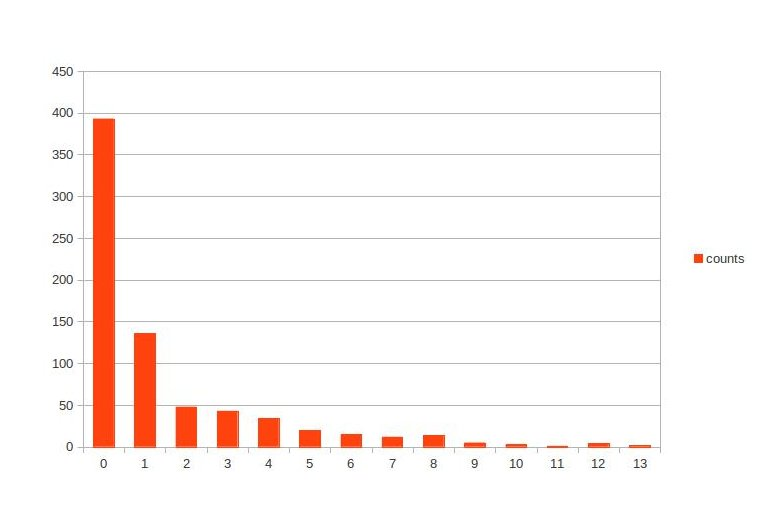
\includegraphics[scale=0.6]{length_based_results_better.jpg}
    \end {center}
    \item word differences:
    \begin{itemize}
        \item \textbf{393} chunks had \textbf{0} difference in words
        \item \textbf{136} chunks where different by \textbf{1} word (missing or additional)
        \item \textbf{48} different by \textbf{2} words
        \item \textbf{56} with a difference over \textbf{5} words
    \end{itemize}
\end{itemize}

\newpage
For \textbf{503} speeches, with a pause longer than \textbf{300ms}:
\begin{itemize}
    \item time differences: \newline
    \begin{itemize}
        \item there were \textbf{154} chunks which time frame were within a \textbf{0.5s} difference, 
        \item average time difference was \textbf{5.24s}
        \item standard deviation was \textbf{5.23s}
        \item maximum time difference was \textbf{37.9s}
    \end{itemize}
    \begin{center}
        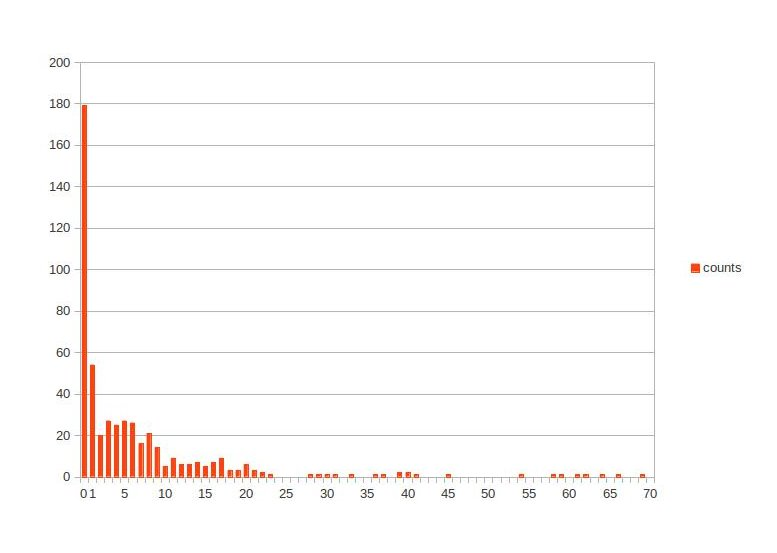
\includegraphics[scale=0.6]{length_based_results_worse.jpg}
    \end {center}
    \item word differences:
    \begin{itemize}
        \item \textbf{179} chunks had \textbf{0} difference in words
        \item \textbf{54} chunks where different by \textbf{1} word (missing or additional)
        \item \textbf{20} different by \textbf{2} words
        \item \textbf{56} with a difference over \textbf{10} words
    \end{itemize}
\end{itemize}

\newpage
\subsection{Conclusions}

The time statistics are showing a bit worse results, because word labels are more precise than chunk time frames. \newline

The results are within expectations, after all it is very crude algorithm. It probably could be improved though, however it is hard without introducing much more knowledge about language and possibly some additional training data (i.e. time of phonemes). \newline

This algorithm is a bit sensitive to a chunks created. If only the longer pauses are allowed, by increasing the holes filling factor from 200ms to 300ms in  speech detection algorithm, the results were considerably worse. \newline
In this case detected speeches contained more silence frames and consequently the total time is different, and the estimated times might be a bit more wrong. Another reason why it produces worse results might be related to the fact, that it also causes the speeches to be on average longer. This kind of random variables follow a rule, that they differ from an estimated value by square root factor, ergo longer parts, worse estimations.

\newpage
\begin{center}
    \section{Audio based alignment}
\end {center}
\subsection{Speech recognition}

Audio based alignment is simplified problem of speech recognition. Usually in speech recognition the language consist of millions of words in different conjugations, which may create many different sentences. In audio alignment we expect only one text and only one sentence at the time. \newline

Usually speech recognition is based on trained Hidden Markov Models with Gaussian Phoneme models, although successful systems rarely rely on single state phoneme model. \newline
As I mentioned before (3.1) there are many different allophones of single phoneme. A variations are largely attributed to surrounding they are spoken in. For example in polish there are softening phonemes 'i' and 'j', that clearly change how preceding or succeeding phonemes are realized. At some contexts it may happen that certain phoneme will lose it voice are even get silent completely, at another they will be strengthened with additional voice, i.e.: 
\begin{description}
	\item[“staw płytki”] $\rightarrow$ “w” loses it voice and starts to remind a phoneme “f”
	\item[“plac budowy”] $\rightarrow$ “c” gains additional voice and reminds a phoneme “dz”
\end{description}
And almost never one can cleanly separate two consecutive phones. \newline

 In order to better model different realisations of phonemes, an audio modelling contains models of phonemes at different triphone contexts. 
For every possible neighbourhood a given phoneme might appear, a separate Gaussian model is trained, for example a WSJ model from sphinx database contains 40 different phonemes and additional silence phoneme, that gives 68921 different triphones, however WSJ model contains over 110k elements,  because of additional information about location within a word. \newline

It is not over yet, because transitioning from phoneme to phoneme should be modelled somehow as well. The obvious solution is to train a triple state HMM, which will better fit the changing phone. \newline
That triples number of states. \newline

This huge number of different models requires a lot of training data, which is on one hand not easy to come along with, on another requires a lot of time to train with. \newline
Training data for speech recognition is one constant problem, which have to be dealt with. The problem is amplified, by the fact, that training samples should be small and very well described. That hardly can be done manually. \newline
Another bad news is, that a model trained on news feeds, is expected to perform poorly as a spoken address recognition software. \newline

\newpage

Once we have our audio model, than speech recognition is an easy piece, isn't it? \newline
Not really, since so many possible and often similar words make it a hard problem. Rarely a speech recognition software is based solely on audio model to recognize a sequence of phonemes. \newline
Problem is, that the number of states is too huge in order to be processed exhaustively, even though we can use a Viterbi algorithm to find a best (most probable) sequence of states for given observation sequence and we keep results only for a present moment in time (a single frame), that still gives a huge number
of kept states with calculated score. \newline

The sphinx library deals with this problem by searching in a breadth first search manner (meaning that it will keep states only from a current moment) and to cut on number of states to process, a priority queue is used, which keeps only best scoring ones. \newline

And this is the part of recognition software we would like to use for the alignment problem. \newline
The difference from here is that, we do know what the text is spoken, while for recognition there is no such knowledge. \newline
However let's dwell on this a little bit longer, so we can see what a huge simplification it makes. \newline

Let's start with a simple example by using WSJ dictionary: \newline
phoneme sequence “W AH N”, which  on it's own can be recognized as word “one” or “won” is also a prefix for 36 another different words and subsequence of total 117 different words. \newline
There is a sequence “W AH N S EH L F”, which assigned to word “oneself”, however it may also be from the end of word “penguin” (“W AH N”) and beginning of word “cellphone” (“S EH L F”). \newline

Sphinx library provides two ways of language modelling to tackle sucha ambiguity:
\begin{itemize}
    \item ngrams frequencies
    \item language grammar
\end{itemize}

For simple languages, like a sequence of digits or language containing one long sequence (like in case of text alignment), it is advisable to use language grammar. \newline
For general recognition software like Apple Siri, ngrams are necessary, although I am not convinced that they haven't used a sort of grammar for typical queries. \newline

Ngrams (in wsj n is maximum 3) are a way to assign a probability to word sequences. In above example it is expected, that “oneself” is more probable to occur in real word, than the later case, although obviously we can't judge so easily, since the probability of choosing these particular word depends on a probability of whole sentence. \newline

Anyway I think that's enough about speech recognition. \newline
For our purposes we need “only” audio model and word to phoneme sequence dictionary, in order to efficiently  align text to speech. \newline

\newpage
\subsection{Differences between english, russian and polish phonetics}

The sets of phonemes for any language differ slightly between publications and they differ even more between different audio models. For that reason I'm not going to introduce here established phonology for any language, however I'll try to match a phoneme set used by WSJ model for English, VoxForge model for Russian, Corpora and mine for Polish. \newline

In the table below I collected phonemes from four used sets and analysed differences, that may cause problem to represent some words using given phonetics and in result may cause problems with alignment. The table is organized so the similar phonemes are next to each other. If there is not alternative in a language, than the row remains empty. \newline

\newcommand{\strutA}[1]{% no space before strut
\rule[0pt]{0pt}{#1}% put text approx mid strut
}


\fontsize{10pt}{12pt}\selectfont
\begin{center}
\begin{tabularx}{\linewidth}{| p{1cm} | p{1.2cm} | p{1cm} | p{1.1cm} | p{1.1cm} | p{1cm} | p{1.1cm} | p{4.9cm} |}
\hline
\rowcolor[gray]{0.8}
English & example & Russian & example & Corpora Polish & Polish used by me & example & Notes on similarities
\\ \hline

AA & ad\underline{o}pt & a & \underline{а}рен\underline{а} & a & a & dwa &
\multirow{3}{\linewidth}{The most different from this set is English „AE”, which also shows a similarity to Polish and Russian „e”} \strutA{2ex}
\\ \cline{1-7}
AE & \underline{a}ct & aa & \underline{а}кт &&&&  \strutA{2ex}
\\ \cline{1-7}
AH & \underline{a}cute &&&&&& \strutA{2ex}
\\ \hline
AW & all\underline{ow} &&& a\_ (ą) && tą & \multirow{2}{\linewidth}{There is no such a vowel in Russian however it can be substituted with „oo l”, similar for my Polish model with „o ł”}  \strutA{4ex}
\\ \cline{1-7}
OW & aer\underline{o} &&&&&& \strutA{4ex}
\\ \hline
AY & b\underline{i}ke &&&&&& Simulated with Russian and Polish „a j”
\\ \hline
B & \underline{b}ill & b & \underline{б}ыл & b & b & \underline{b}yć & Quite similar
\\ \hline
&& bb & де\underline{б}ет &&&& A softened version of „b”, a bit different, but Polish and English „b”  can also be slightly softened
\\ \hline
&& c & \underline{ц}вет & c & c & \underline{c}oś & In English it is something like \newline „T S”
\\ \hline
CH & jackovi\underline{ch} & ch & дево\underline{ч}ка & ci (ć) & ć & czci\underline{ć} & 
\multirow{2}{\linewidth}{English „CH” is actually used for slavian words containing „c”, „ć”, „cz” like phonemes. Russian „ch” is similar to softened Polish „cz”, so it has to replace both „ć” and „cz”} \strutA{6ex}
\\ \cline{1-7}
&&&& cz & cz & \underline{cz}ego & \strutA{7ex}
\\ \hline
JH & \underline{j}ust &  &  & drz &  & \underline{dż}em & Simulated by „d zh” or „d ż”, English „JH” is quite similar.
\\ \hline
 &  &  &  & dzi (dź) &  & ka\underline{dź} & Simulated by „d zh” or „d ź”, English „JH” must simulate this one as well, although it also can be softened, it is not very similar.
\\ \hline
D & \underline{d}a\underline{d} & d & \underline{д}лина & d & d & \underline{d}uży & \multirow{2}{\linewidth}{Except for Russian and Polish „d”, all are a bit different. „dd” is again a softened version.}  \strutA{1ex}
\\ \cline{1-7}
 &  & dd & \underline{д}итя &  &  & & \strutA{1ex}
\\ \hline
DH & \underline{th}ey &  &  &  &  &  & No counterparts, something between „d” and „z”.
\\ \hline
\end{tabularx}
\end{center}

\newpage

\begin{center}
\begin{tabularx}{\linewidth}{| p{1cm} | p{1.2cm} | p{1cm} | p{1.1cm} | p{1.1cm} | p{1cm} | p{1.1cm} | p{4.9cm} |}
\hline
\rowcolor[gray]{0.8}
English & example & Russian & example & Corpora Polish & Polish used by me & example & Notes on similarities
\\ \hline
 &  &  &  & e\_ (ę) &  & s\underline{ę}k & Like „ee l” or „e ł” or „EH W”
\\ \hline
EH & thr\underline{ea}d & e & диван\underline{е} & e & e & \underline{e}la & \multirow{2}{\linewidth}{Similary as „a” alternatives, all sound quite alike, but a bit different. Russian differs in a stress, English „ER” is an "e" merged with a silent „r”} \strutA{5ex}
\\ \cline{1-7}
ER & thrill\underline{er} & ee & дн\underline{е} &  &  &  & \strutA{5ex}
\\ \hline
EY & thursd\underline{ay} &  &  &  &  &  & Like „e j”.
\\ \hline
F & \underline{f}ilm & f & \underline{ф}азы & f & f & \underline{f}ilm & \multirow{2}{\linewidth}{Very alike, except of course a softened Russian version}
\\ \cline{1-7}
&& ff & \underline{ф}илат &&&& 
\\ \hline
G & ea\underline{g}er & g & дол\underline{г}о & g & g & \underline{g}ęś & \multirow{2}{\linewidth}{As above}
\\ \cline{1-7}
&& gg & дол\underline{г}е &&&& 
\\ \hline
HH & \underline{wh}o & h & дома\underline{х} & h & h & \underline{ch}ata & \multirow{2}{\linewidth}{As above}
\\ \cline{1-7}
&& hh & ду\underline{х}и &&&& 
\\ \hline
IH & p\underline{i}cture & i & духам\underline{и} & i & i & \underline{i}gła & \multirow{2}{\linewidth}{Russian and English variations differ in stress, but all are quite similar} \strutA{2ex}
\\ \cline{1-7}
IY & acr\underline{ee} & ii & дух\underline{и} &  &  &  & \strutA{2ex}
\\ \hline
 &  & ae & ран\underline{я}т &  &  &  & This is a quite like „i” phoneme, but not completely. In Russian many vowels can be shortened to unrecognized version, which sounds like „i”.
\\ \hline
K & \underline{q}uote & k & \underline{к}афедр & k & k & \underline{k}to & \multirow{2}{\linewidth}{Very alike, except of course a softened Russian version.} \strutA{2ex}
\\ \cline{1-7}
 &  & kk & \underline{к}ефир &  &  &  & 
\\ \hline
Y & la\underline{wy}er & j & рано\underline{й} & j & j & \underline{j}ak & Very similar.
\\ \hline
L & \underline{l}awyer & ll & а\underline{л}екс & l & l & \underline{l}ato & Quite similar, although Russian is a softened version of „l”, so it doesn't cover all allophones of Polish „l”
\\ \hline
W & \underline{w}ork & l & \underline{л}ад & l\_ (ł) & ł & \underline{ł}ąka & Quite similar
\\ \hline
M & \underline{m}o\underline{m} & m & \underline{м}алы & m & m & \underline{m}a\underline{m}a & 
\multirow{2}{\linewidth}{Very alike, except of course a softened Russian version}
\\ \cline{1-7}
 &  & mm & малы\underline{м}и &  &  &  & 
\\ \hline
N & \underline{n}ail & n & \underline{н}адеюсь & n & n & \underline{n}os & Very alike.
\\ \hline
 &  & nn & наде\underline{нь} & ni (ń) & ń & ko\underline{ń} & No English alternatives, although it seems reasonable to use „N Y” sequence.
\\ \hline
NG & thi\underline{ng} &  &  &  &  &  & In Russian and Polish might be simulated with „n g” or just „n”, but no natural alternatives
\\ \hline
AO & f\underline{o}r & oo & подн\underline{ё}с & o & o & t\underline{o}k & Quite similar
\\ \hline
 &  & ay & п\underline{о}гадай &  &  &  & Non stressed version of „oo”, however it sounds more like „a”
\\ \hline
OY & foil &  &  &  &  &  & Can be simulated with „o i”.
\\ \hline
P & \underline{p}ack & p & \underline{п}оезд & p & p & \underline{p}as & 
\multirow{2}{\linewidth}{Similar. Russian allophones cover Polish and English phonemes.} \strutA{2ex}
\\ \cline{1-7}
 &  & pp & пом\underline{п}е &  &  &  & \strutA{2ex} 
\\ \hline
R & \underline{r}ace & r & \underline{р}ад & r & r & \underline{r}u\underline{r}a & \multirow{2}{\linewidth}{As above}
\\ \cline{1-7}
 &  & rr & \underline{р}юкзак &  &  &  & 
\\ \hline
S & \underline{s}and & s & \underline{с}цен & s & s & \underline{s}en &  \multirow{2}{\linewidth}{As above}
\\ \cline{1-7}
 &  & ss & \underline{с}егодня &  &  &  & 
\\ \hline
\end{tabularx}
\end{center}

\newpage

\begin{center}
\begin{tabularx}{\linewidth}{| p{1cm} | p{1.2cm} | p{1cm} | p{1.1cm} | p{1.1cm} | p{1cm} | p{1.1cm} | p{4.9cm} |}
\hline
\rowcolor[gray]{0.8}
English & example & Russian & example & Corpora Polish & Polish used by me & example & Notes on similarities
\\ \hline
SH & \underline{sh}op & sh & \underline{ш}ёлка & si & ś & \underline{ś}liwka & Quite alike.
\\ \hline
 &  &  &  & sz & sz & \underline{sz}osa & It is a bit similar to "ś", but no real alternatives.
\\ \hline
 &  & sch & \underline{щ}ека &  &  &  & No real counterpart. Can be simulated with „SH CH” and „ś ć' or „sz cz” and variations
\\ \hline
T & \underline{t}in & t & \underline{т}а & t & t & \underline{t}en & 
\multirow{2}{\linewidth}{Similar. Russian allophones cover Polish and English phonemes.} \strutA{2ex}
\\ \cline{1-7}
 &  & tt & \underline{т}ёмный &  &  &  & \strutA{2ex}
\\ \hline
TH & \underline{th}anks &  &  &  &  &  & No counterparts, something between „f” and „t”.
\\ \hline
UH & f\underline{oo}t & u & ёлк\underline{у} & u & u & \underline{ó}semka &
\multirow{3}{\linewidth}{All are quite alike, although subtle differences remain.}
\\ \cline{1-7}
UW & f\underline{oo}l & ur & \underline{ю}г &  &  &  & 
\\ \cline{1-7}
 &  & uu & абсол\underline{ю}т &  &  &  & 
\\ \hline
V & \underline{v}isit & v & \underline{в}аза & w & w & \underline{w}iedza &
\multirow{2}{\linewidth}{Similar. Russian allophones cover Polish and English phonemes.} \strutA{2ex}
\\ \cline{1-7}
 &  & vv & жи\underline{вь}ем &  &  &  & \strutA{2ex} 
\\ \hline
 &  & y & жив\underline{ы} & y & y & d\underline{y}m &
\multirow{2}{\linewidth}{Russian allophones differ in stress, but there is a problem with English equivalent. The most alike phoneme is „IH”.} \strutA{4ex}
\\ \cline{1-7}
 &  & yy & жив\underline{ы}х &  &  &  & \strutA{4ex} 
\\ \hline
Z & vi\underline{s}or & z & ва\underline{з}а & z & z & \underline{z}ebra & Quite alike.
\\ \hline
 &  & zz & ва\underline{з}е & zi (ź) & ź & \underline{ź}le & Russian and Polish are very alike. No English equivalent, „ZH” is the closest.
\\ \hline
ZH & vi\underline{s}ual & zh & \underline{ж}аба & rz (ż) & ż & \underline{rz}eka & Quite alike.
\\ \hline
\end{tabularx}
\end{center}

I can try to draw some conclusions from the table alone. \newline

In English there are no natural alternatives in 8 cases, while in Russian only in 2 cases, although there are some other dissimilarities, it is clearly visible now (if it wasn't before), that Russian is much more similar language to Polish, than English. \newline
It might be a surprise though, that English isn't so different, and it seems possible to emulate every Polish word with English phonemes.
Maybe not too surprising though, after all we are all humans.

\newpage
\subsection{Grapheme to phoneme conversion grammar}

For the purpose of speech recognition we require very accurate dictionaries, that keep track of actual pronunciation of words with all possible variations. \newline

Usually the dictionaries are created by analysing actual recordings. \newline
I would like to propose a way of converting grapheme sequences into phonetic description, which might be good enough for many real life applications, like word alignment or even phoneme alignment. \newline
Nevertheless it would still be applicable only to problems which are easier than speech recognition, but only because it is a hard problem, which tries to get as much accuracy from sub-problems as it is only possible. \newline

Take a look at English  word “one” and “tone”. The differ with character, but a phonectics are: “W AH N”  and “T OW N”.  \newline
It doesn't seem to be trivial, but for Polish language it might be easy enough to create such a grammar, that creates such a dicitionary with good enough accurracy.

We need at least three of such a grammars, converting to English, Russian and Polish phonemes.


 Here are example conversions:

\fontsize{12pt}{14pt}\selectfont
\newpage

\begin{center}
\begin{tabular}{| p{8cm} | p{8cm} |}
\hline
\rowcolor[gray]{0.8}
synthesized texts &
Notes on erroneous parts in synthesized speech using words and phonemes initiated by pause based alignment
\\ \hline
"Rosja przedwojenna była wymarzoną areną dorobku dla ludzi tego typu zwłaszcza pochodzących z Królestwa" &
- „areną” – „a” is missing \newline
- jumps between phonemes are clearly visible, although they are not disturbing enough to cloud the meaning
\\ \hline
"Wiadomości zaczerpnięte w klasach gimnazjalnych wrodzona inteligencja która wraz ze zdrowiem towarzyszyła poszukiwaczowi posady i na zawołanie zjawiała się nie siana i nie pielęgnowana wytrzymałość odwaga wesołość i pewna odrobina drwiny z Moskala u którego się służy lecz nad którym jednak panuje się mimo wszystko torowały drogę od niższej do wyższej pozycji" &
- the phonemes of word „mimo” are quite short, so listener need to be really focused, to not miss a meaning of the word, \newline
- after „zjawiała się” there are two extra words „do wyjścia”,
closer inspections showed, that „się” was included as whole, but was badly aligned,
\\ \hline
"Trzeba przyznać że nie ostatnią rolę grała w tej operze protekcja cicha pokorna dobra wróżka prowadząca za rękę od niskiego do coraz wyższego rodaka tu i tam zaczepionego nogą lub łokciem na tej rosyjskiej drabinie" &
- „przyznać” - „ć” is actually „ź” \newline
- „tej” is something else \newline
- „protekcja” - hearable „w” before „t” \newline
- „spokojna” - something extra after „k” \newline
- „zaczepionego” - „z” is missing \newline
- „drabinie” - „ie” is missing \newline
\\ \hline
"Chrząszcz brzmi w trzcinie w Szczebrzeszynie W szczękach chrząszcza trzeszczy miąższ Czcza szczypawka czka w Szczecinie" &
- „brzmi” - „żm” phoneme sequence was not found in whole text so it was omitted in the synthesized audio, \newline
- „czcza” sounds like „cza”, \newline
- „Szczecinie” - „ie” missing
\\ \hline
"Chrząszcza szczudłem przechrzcił wąż Strząsa skrzydła z dżdżu A trzmiel w puszczy, tuż przy Pszczynie Straszny wszczyna szum" &
- „wąż” - „ą” is missing \newline
- „straszny” - „ny” is missing \newline
- „szum” - „m” is strange
\\ \hline
"Litwo Ojczyzno moja ty jesteś jak zdrowie Ile cię trzeba cenić ten tylko się dowie Kto cię stracił Dziś piękność twą w całej ozdobie Widzę i opisuję bo tęsknię po tobie" &
- „cenić” - „ć” is missing \newline
- „stracił” - extra „e” or even kind of „em” \newline
- „piękność” - very short „e” \newline
- „ozdobie” - first „o” is missing, second sounds like „ą” \newline
- „tobie” - short „e”
\\ \hline
\end{tabular}
\end{center}

\newpage

\begin{center}
\begin{tabular}{| p{8cm} | p{8cm} |}
\hline
\cellcolor[gray]{0.8}
synthesized texts &
\cellcolor[gray]{0.8}
Notes on erroneous parts in synthesized speech using words and phonemes initiated by pause based alignment
\\ \hline
"Panno święta co Jasnej bronisz Częstochowy I w Ostrej świecisz Bramie Ty co gród zamkowy Nowogródzki ochraniasz z jego wiernym ludem" &
- „świecisz” - „ś” sounds weird like "sz" through teeth, \newline
- „co” - hearable „t” at end, \newline
- „gród” - missing „g”, \newline
- „nowogródzki” - extra „na” at the beginnings and „dz” sounds like „jz”, \newline
- „ochraniasz” - first „o” is actually „w”, \newline
- „wiernym” - quite bad, at the beginning there is extra „pły”, and there is missing „r” making it completely unrecognizeable
\\ \hline
"Jak mnie dziecko do zdrowia powróciłaś cudem Gdy od płaczącej matki, pod Twoją opiekę Ofiarowany martwą podniosłem powiekę I zaraz mogłem pieszo do Twych świątyń progu Iść za wrócone życie podziękować Bogu Tak nas powrócisz cudem na Ojczyzny łono" &
- „mnie” - extra „u” at the beginning, \newline
- „ofiarowany” - first „o” sounds like „he”
\\ \hline
"Tymczasem przenoś moją duszę utęsknioną Do tych pagórków leśnych, do tych łąk zielonych Szeroko nad błękitnym Niemnem rozciągnionych" &
- „łąk” - extra short „a” at the beginning
\\ \hline
"Do tych pól malowanych zbożem rozmaitem Wyzłacanych pszenicą, posrebrzanych żytem Gdzie bursztynowy świerzop, gryka jak śnieg biała Gdzie panieńskim rumieńcem dzięcielina pała" &
- „do” - extra „łe” at the end, \newline
- „rozmaitem” - sounds like „smeitem”, \newline
- „gryka” - noticeable short „ł” at the end, \newline
- „panieńskim” - „ie” is short, \newline
- „rumieńcem” - a pause between „m” and „ie”
\\ \hline
"A wszystko przepasane jakby wstęgą miedzą Zieloną na niej z rzadka ciche grusze siedzą" &
- „wstęgą” - only „gą” is recognizeable
\\ \hline
"na stole z powyłamywanymi nogami leżą śliwki czereśnie pomarańcze i ogórki" &
- „leżą” - extra „na” up front, \newline
- „czereśnie” - missing „re”
\\ \hline
"W czasie suszy szosa sucha" &
\\ \hline
"Za górami za lasami znajduję się wysoka wieża strzeżona przez smoka" &
\\ \hline
\end{tabular}
\end{center}

\newpage

\begin{center}
\begin{tabular}{| p{8cm} | p{8cm} |}
\hline
\cellcolor[gray]{0.8}
synthesized texts &
\cellcolor[gray]{0.8}
Notes on erroneous parts in synthesized speech using words and phonemes initiated by pause based alignment
\\ \hline
"Maksymalistyczny egzystencjalny program Mrożka polegał właśnie na stawianiu świata pod znakiem zapytania w świetle jak najbardziej trzeźwych zarzutów o jego niewystarczalność" &
- „maksymalistyczny” - first „m” is actually an „s”, extra „lny” at the end, \newline
- „mrożka” - „first „m” is actually „z”, \newline
- „polegał” - extra short trailing „o”, \newline
- „o” - very short and faint
\\ \hline
"Mrożek jako krytyk cywilizacji widział w niej nadto przemoc mechanizm mielenia jednostek na proszek W rewolucjach brzydził go fetor mierzwy w jaką zmieniają się górnolotne czyste ideały" &
- „mechanizm”- sounds like „mechaniźmie”, because „z” is „ź”, \newline
- „jednostek” - short but loud extra „w” at the beginning, \newline
- „brzydził” - noticeable „g” between „y” and „dz”, \newline
- „fetor” - trailing „e”, \newline
- „ mierzwy” - missing „y”, \newline
- „jaką” - a bit distorted and unrecognizeable, \newline
- „ideały” - „i” is replaced by „u” and extra „j” between „e” and „a”

\\ \hline
"Pomimo języka groteski którym tak chętnie się posługiwał był przede wszystkim piewcą głębi sztuki jej ocalającego kontemplacyjnego wymiaru" &
- „pomimo” - some artefact in ending „o”, \newline
- „jej” - something extra at the beginning, \newline
- „ocalającego” - some „r” after „oca”

\\ \hline
"Przy czym nigdy głośno o tym nie mówił Jednocześnie sceptycznie i ostrożnie podchodził do kwestii wyobraźni widząc w niej zasadę kierującą ludzkimi poczynaniami a co z kolei skutkuje każdorazowo totalitarną eksterminacją" &
- „kwestii” - last „i” like „j”, \newline
- „wyobraźni” - missing „ob” changing the meaning of the word, \newline
- „totalitarną” - „ą” sounds like „ąu”

\\ \hline
\end{tabular}
\end{center}
\newpage
\begin{center}
    \section{Bibliography}
\end {center}

\begin{thebibliography}{99}
\bibitem{englishDict} Houghton Mifflin Company. \emph{The American Heritage Dictionary of the English Language}, Fourth Edition, 2000.
\bibitem{albertiiAnatomy} Prof. W. Alberti. \emph{The anatomy and physiology of the ear and hearing.}
\bibitem{piconeFundamentals} Prof. Joseph Picone \emph{Fundamentals of speech recognition}
\bibitem{olsonMusic} Olson Harry F. (1967) \emph{Music, Physics and Engineering}
\bibitem{volkman} Stevens Stanly Smith, Volkman John, Newman Edwin B. (1937) \emph{A scale for the measurement of the psychological magnitude pitch Journal of the Acoustical Society of America}
\bibitem{douglasCommunication} Douglas O'Shaughnessy (1987) \emph{Speech communication: human and machine.}
\bibitem{zwicker} Zwicker E. (1961) \emph{Subdivision of the audible frequency range into critical bands.}
\bibitem{melCepstrum} H.P. Combrinck and E.C. Botha \emph{On The Mel-scaled Cepstrum}
\bibitem{welchFFT} Welch P. (1967) \emph{The use of fast Fourier Transform for the estimation of power spectra: A method based on time averaging over short, modified periodograms}
\bibitem{smithDigital} Steven W. Smith \emph{The scientist and engineer's guide to digital signal processing.}
\bibitem{} A. Pinsky \emph{Introduction to Fourier analysis and wavelets}
\bibitem{} B.P. Bogert, M. J. R. Healy, J. W. Tukey \emph{The Quefrency Alanysis of Time Series for Echoes: Cepstrum, Psuedo-Autocovariance, Cross-cepstrum and Saphe Cracking }
\bibitem{} Seyed Hamidreza Mohammadi, Hossein Sameti, Amirhossein Tavanaei, Ali Soltani-Farani \emph{Filter-bank design based on dependencies between frequency components and phonem characteristic}
\bibitem{} Dr. James Glass, prof. Victor Zue \emph{Automatic Speech Recognition} MIT course.
\bibitem{} Daniel Jurafsky, James H. Martin \emph{Speech and language processing}
\bibitem{} B. Plannerer \emph{An Introduction to Speech Recognition }
\bibitem{} Davis, Marmelstein (1980) \emph{Comparison of parametric representation of monosyllable word recognition in continously spoken sentences}
\bibitem{} Ahmed N., Natarjan T., Rao K.R. (1974) \emph{Discrete Cosine Transform}
\bibitem{} Syed Ali Khayam \emph{The Discrete Cosine Transform (DCT): Theory and Application} 
\bibitem{} Crystal David \emph{Linguistic}
\bibitem{} Chomsky N., Halle M. \emph{The sound pattern of English}
\bibitem{} Jagodziński G. \emph{Gramatyka języka polskiego.}
\bibitem{} J.L. Rodgers, W.A.Nicewander \emph{Thirteen ways to look at the correlation coefficient.}
\bibitem{} Jae Myung \emph{Tutorial on maximum likelihood estimation}
\bibitem{} Prof. A. Moore \emph{Clustering with Gaussian Mixtures}
\bibitem{} Jeff A. Bilmes \emph{A Gentle Tutorial of the EM Algorithm and its Application to Parameter Estimation for Gaussian Mixture and Hidden Markov Models}
\bibitem{} M. Karaś, M. Madejowa \emph{Słownik wymowy polskiej.}
\bibitem{} John-Paul Hosom \emph{Speaker-Independent Phoneme Alignment Using Transition- Dependent States}
\end{thebibliography}

\end{document}
